\documentclass[conference]{IEEEtran}
\IEEEoverridecommandlockouts
\usepackage{cite}
\usepackage{amsmath,amssymb,amsfonts}
\usepackage{algorithmic}
\usepackage{graphicx}
\usepackage{textcomp}
\usepackage{xcolor}
\usepackage{booktabs}
\usepackage{array}
\usepackage{tabularx}
\usepackage{multirow}
\usepackage{hyperref}
\usepackage{balance}
\usepackage{tikz}
\usetikzlibrary{shapes.geometric,arrows.meta,positioning,fit,backgrounds,calc}

\begin{document}

\title{Decoding Crime Narratives Using NLP and Big Data Analytics: A Reproducible Spark, BERT, CRF, Topic-Modelling and Semantic-Retrieval Framework}

\author{
\IEEEauthorblockN{Avusali Vivek Chary}
\IEEEauthorblockA{Amrita School of AI\\
Amrita Vishwa Vidyapeetham\\
Faridabad, India\\
dl.ai.u4aid24010@dl.students.amrita.edu}
\and
\IEEEauthorblockN{Mayank Thukran}
\IEEEauthorblockA{Amrita School of AI\\
Amrita Vishwa Vidyapeetham\\
Faridabad, India\\
dl.ai.u4aid24023@dl.students.amrita.edu}
\and
\IEEEauthorblockN{Bhamidi Naga Sai Surya Bharadwaj}
\IEEEauthorblockA{Amrita School of AI\\
Amrita Vishwa Vidyapeetham\\
Faridabad, India\\
dl.ai.u4aid24012@dl.students.amrita.edu}
\and
\IEEEauthorblockN{Mr. Suraj Singh}
\IEEEauthorblockA{School of AI\\
Amrita Vishwa Vidyapeetham\\
Faridabad, India\\
alok.srivastava@dl.amrita.edu}
}
\maketitle

\begin{abstract}
Unstructured incident narratives contain document-level categories, participant roles, locations, objects, temporal references and evidence descriptions that are difficult to aggregate using conventional tabular analytics. This paper presents an end-to-end Natural Language Processing (NLP) and Big Data Analytics framework for converting fictional English crime narratives into structured, searchable and explainable information. The system generates a reproducible corpus of 60,000 valid reports and 2,700 controlled faulty records, cleans and deduplicates them using Apache Spark, and stores the resulting data as split-partitioned Parquet. It compares Bag-of-Words, TF--IDF, averaged Word2Vec and compact BERT document classifiers; compares a linear-chain Conditional Random Field (CRF) with a fine-tuned BERT token classifier for eight entity types; and applies LDA/NMF topic modelling, spaCy linguistic analysis, VADER polarity, TextRank summarisation and MiniLM semantic retrieval. Validation data control checkpoint selection, confidence calibration and entity-model selection; model hashes are frozen before final-test evaluation. The processed corpus is enriched into Parquet, SQLite, sparse lexical indexes and dense semantic indexes that support a seven-page Streamlit dashboard. On the fixed synthetic test sample, Word2Vec achieved 95.17\% document accuracy, TF--IDF achieved 83.67\%, compact BERT achieved 83.25\%, and the validation-selected CRF reached 98.46\% strict entity F1. These results demonstrate the integration of classical and neural NLP with reproducible Spark engineering, while not constituting evidence of performance on real police narratives.
\end{abstract}

\begin{IEEEkeywords}
natural language processing, Apache Spark, crime narratives, text classification, named entity recognition, BERT, conditional random field, topic modelling, semantic search, Streamlit
\end{IEEEkeywords}

\section{Introduction}

Narrative reports preserve contextual information that is commonly lost when events are reduced to fixed database columns. A single narrative may describe an alleged event, distinguish a victim from a suspect, identify a location and property, mention a weapon under negation, record a time, and cite evidence. Manually examining tens of thousands of such documents is slow and inconsistent; simple keyword counts also fail to represent context, grammatical role and semantic similarity.

The objective of this work is to build a reproducible system that transforms a large narrative corpus into document labels, typed spans, topics, summaries, linguistic annotations and searchable representations. For a narrative $x$, the system produces
\begin{equation}
\mathcal{A}(x)=
\{\hat{y},p,\mathcal{E},\theta,s_{\mathrm{pol}},s_{\mathrm{cue}},
\mathcal{S},\mathcal{G},\mathcal{R}\},
\end{equation}
where $\hat{y}$ is the predicted category, $p$ is calibrated confidence, $\mathcal{E}$ contains typed spans, $\theta$ is a topic distribution, $s_{\mathrm{pol}}$ is polarity, $s_{\mathrm{cue}}$ is a transparent cue score, $\mathcal{S}$ is a summary, $\mathcal{G}$ is grammatical analysis and $\mathcal{R}$ is retrieved evidence.

The project uses fictional data to demonstrate NLP and distributed engineering without presenting generated records as genuine police data. Its contributions are:
\begin{itemize}
\item \textbf{Reproducible Corpus:} 60,000 unique labelled narratives across eight categories and 384 scenario groups, plus controlled quality faults.
\item \textbf{Spark Pipeline:} schema validation, deterministic hash deduplication, partitioned Parquet, SQL trends and an MLlib baseline.
\item \textbf{Comparative NLP:} shared evaluation for BoW, TF--IDF, Word2Vec and BERT classification, and CRF versus BERT entity extraction.
\item \textbf{Leakage-Aware Evaluation:} group-separated splits, validation-only selection and calibration, model hashes and final-test receipts.
\item \textbf{Searchable Application:} keyword, MiniLM semantic and reciprocal-rank hybrid search connected to SQLite and Streamlit.
\item \textbf{Responsible Interpretation:} explicit limitations, negation-aware mentions, heuristic redaction and separation of polarity from threat cues.
\end{itemize}

\section{Literature Review}

The framework combines established work from distributed analytics, text representation, contextual modelling, structured prediction and retrieval. Spark provides a unified distributed engine for structured processing and machine learning~\cite{zaharia2016spark}. Word2Vec learns distributed lexical representations from local context~\cite{mikolov2013}. BERT introduced deep bidirectional Transformer pretraining followed by task-specific fine-tuning~\cite{devlin2019}. Conditional Random Fields model probabilities over complete label sequences~\cite{lafferty2001}. Latent Dirichlet Allocation discovers document-topic mixtures~\cite{blei2003}, while TextRank uses graph ranking for unsupervised extraction~\cite{mihalcea2004}. Sentence-BERT supports efficient semantic similarity~\cite{reimers2019}, and VADER provides lexicon-and-rule polarity analysis~\cite{hutto2014}.

\begin{table*}[t]
\centering
\caption{Foundational Literature and Positioning of the Proposed Framework}
\label{tab:litreview}
\renewcommand{\arraystretch}{1.25}
\small
\begin{tabularx}{\textwidth}{|p{2.5cm}|X|X|X|}
\hline
\textbf{Reference} & \textbf{Core contribution} & \textbf{Limitation relative to this project} & \textbf{Use in this work}\\
\hline
Zaharia et al.~\cite{zaharia2016spark} & Unified distributed engine for batch, SQL and ML. & Does not define a narrative-specific pipeline. & DataFrame validation, SQL, deterministic deduplication, Parquet and MLlib.\\
\hline
Mikolov et al.~\cite{mikolov2013} & Efficient neural word representations. & Word vectors do not directly yield document labels. & Training-only skip-gram vectors are averaged and classified by logistic regression.\\
\hline
Devlin et al.~\cite{devlin2019} & Bidirectional Transformer pretraining. & Greater complexity does not guarantee superiority on every corpus. & Compact BERT is fine-tuned for both document and token classification.\\
\hline
Lafferty et al.~\cite{lafferty2001} & Conditional sequence modelling. & Requires engineered observations and labelled sequences. & A CRF predicts eight BIO entity types using contextual token features.\\
\hline
Blei et al.~\cite{blei2003}; Mihalcea and Tarau~\cite{mihalcea2004} & Topic mixtures and graph-based ranking. & Outputs require interpretation and may omit context. & LDA/NMF expose themes and TextRank returns extractive summaries.\\
\hline
Reimers and Gurevych~\cite{reimers2019} & Efficient sentence embeddings. & General embeddings are not calibrated on project relevance labels. & MiniLM vectors support semantic retrieval and cited evidence selection.\\
\hline
\end{tabularx}
\end{table*}

\begin{figure}[t]
\centering
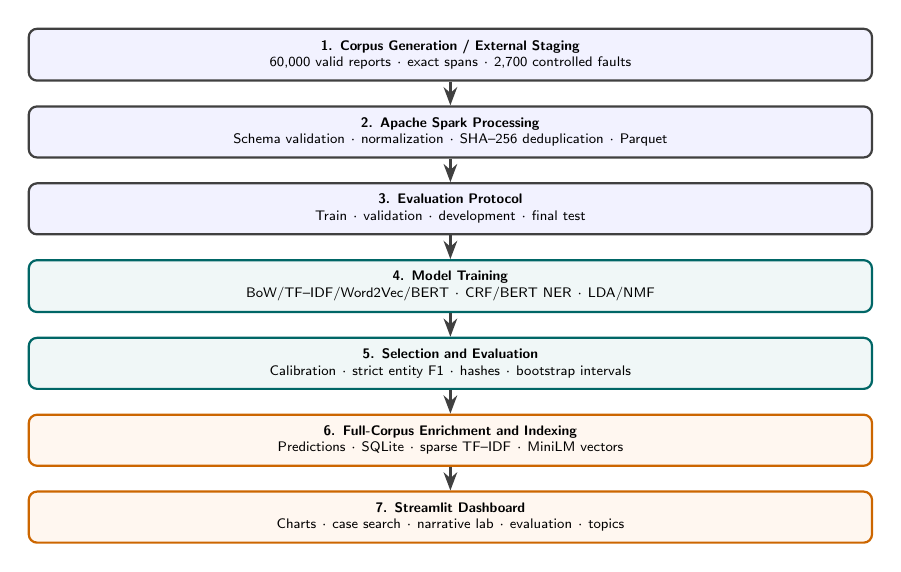
\begin{tikzpicture}[
  node distance=0.30cm,
  box/.style={draw=black!75,fill=blue!5,rounded corners=3pt,thick,
    align=center,font=\sffamily\tiny,inner sep=4pt,
    text width=0.86\columnwidth,minimum height=0.58cm},
  modelbox/.style={draw=teal!80!black,fill=teal!6,rounded corners=3pt,thick,
    align=center,font=\sffamily\tiny,inner sep=4pt,
    text width=0.86\columnwidth,minimum height=0.62cm},
  outbox/.style={draw=orange!80!black,fill=orange!6,rounded corners=3pt,thick,
    align=center,font=\sffamily\tiny,inner sep=4pt,
    text width=0.86\columnwidth,minimum height=0.58cm},
  arrow/.style={->,>=Stealth,thick,draw=black!75}
]
\node[box] (generate) {\textbf{1. Corpus Generation / External Staging}\\
60,000 valid reports $\cdot$ exact spans $\cdot$ 2,700 controlled faults};
\node[box, below=of generate] (spark) {\textbf{2. Apache Spark Processing}\\
Schema validation $\cdot$ normalization $\cdot$ SHA--256 deduplication $\cdot$ Parquet};
\node[box, below=of spark] (split) {\textbf{3. Evaluation Protocol}\\
Train $\cdot$ validation $\cdot$ development $\cdot$ final test};
\node[modelbox, below=of split] (train) {\textbf{4. Model Training}\\
BoW/TF--IDF/Word2Vec/BERT $\cdot$ CRF/BERT NER $\cdot$ LDA/NMF};
\node[modelbox, below=of train] (evaluate) {\textbf{5. Selection and Evaluation}\\
Calibration $\cdot$ strict entity F1 $\cdot$ hashes $\cdot$ bootstrap intervals};
\node[outbox, below=of evaluate] (enrich) {\textbf{6. Full-Corpus Enrichment and Indexing}\\
Predictions $\cdot$ SQLite $\cdot$ sparse TF--IDF $\cdot$ MiniLM vectors};
\node[outbox, below=of enrich] (dashboard) {\textbf{7. Streamlit Dashboard}\\
Charts $\cdot$ case search $\cdot$ narrative lab $\cdot$ evaluation $\cdot$ topics};
\draw[arrow] (generate) -- (spark);
\draw[arrow] (spark) -- (split);
\draw[arrow] (split) -- (train);
\draw[arrow] (train) -- (evaluate);
\draw[arrow] (evaluate) -- (enrich);
\draw[arrow] (enrich) -- (dashboard);
\end{tikzpicture}
\caption{Top-to-bottom operational pipeline of the crime-narrative analytics framework.}
\label{fig:pipeline}
\end{figure}

\section{Proposed End-to-End Methodology}

The system is organised into seven stages, as illustrated in Fig.~\ref{fig:pipeline}. The command-line controller supports complete execution or individual stages and records status, timing, package versions and content hashes.

\subsection{Stage 1: Reproducible Corpus Generation and Annotation}

The seeded generator creates eight balanced categories: Arson, Assault, Burglary, Cybercrime, Fraud, Robbery, Theft and Vandalism. Eight event variants and six sentence layouts produce
\begin{equation}
8\times8\times6=384
\end{equation}
composite scenario groups. Names, places, objects, weapons and evidence are varied independently. Reports may include unknown or multiple suspects, multiple victims, negated weapons, spelling noise and follow-up paragraphs.

Entity offsets are created during template rendering. For an entity $e_j=(s_j,e_j,l_j,t_j)$, the invariant
\begin{equation}
x[s_j:e_j]=t_j
\end{equation}
ensures that the stored span exactly matches the original narrative. The labels are SUSPECT, VICTIM, LOCATION, WEAPON, PROPERTY, DATE, TIME and EVIDENCE.

The generator writes 60,000 valid reports, then adds 1,500 duplicates, 600 null narratives, 300 blank narratives and 300 invalid dates. An optional importer validates external JSONL in a separate quarantine-aware staging area and records provenance; it does not merge external data into the benchmark automatically.

\subsection{Stage 2: Distributed Spark Validation and Cleaning}

Spark reads 62,700 JSONL rows using an explicit schema and eight partitions. It removes missing required fields, blank text, invalid timestamps, unsupported categories and invalid split values. Original narrative text is retained for entity offsets; a separate lowercase and punctuation-normalised \texttt{clean\_text} column is created.

Normalized text is hashed:
\begin{equation}
h_i=\mathrm{SHA256}(\mathrm{clean\_text}_i).
\end{equation}
A window partitioned by $h_i$ and ordered by report identifier retains one deterministic canonical row. The 60,000 clean rows are written as Parquet partitioned by split. Spark SQL generates month--category--district trends, while a physical plan and data-quality receipt provide execution evidence.

An independent MLlib baseline applies
\begin{equation}
\mathrm{Tokenizer}\to\mathrm{StopWords}\to
\mathrm{HashingTF}\to\mathrm{IDF}\to\mathrm{LogisticRegression}.
\end{equation}
It uses 4,096 hashed features and achieves 87.49\% accuracy on the full Spark test partition.

\subsection{Stage 3: Leakage-Aware Evaluation Protocol}

For every category, incident variants 0--4 are training data, variant 5 is validation, variant 6 is development and variant 7 is final test. First-name pools and participant phrases are also split-specific. The code asserts that no \texttt{template\_group} occurs in multiple splits.

The document experiment uses 6,400 training, 800 validation, 800 development and 1,200 final-test reports. NER uses 3,200 training, 400 validation and 600 final-test reports. Vectorizers and Word2Vec are fitted only on training data. Validation selects BERT checkpoints, temperature and the automatic NER model. SHA--256 hashes are recorded before final-test predictions.

\subsection{Stage 4: Document Representation and Classification}

\subsubsection{Bag of Words and TF--IDF}
Bag of Words uses unigram and bigram counts. TF--IDF additionally discounts globally common terms:
\begin{align}
\mathrm{tfidf}(t,d)&=\mathrm{tf}(t,d)\,\mathrm{idf}(t),\\
\mathrm{idf}(t)&=\log\left(\frac{N+1}{\mathrm{df}(t)+1}\right)+1.
\end{align}
Both use at most 12,000 features and multinomial logistic regression:
\begin{equation}
P(y=c\mid x)=
\frac{\exp(w_c^\top x+b_c)}
{\sum_k\exp(w_k^\top x+b_k)}.
\end{equation}
TF--IDF is the dashboard default because it combines efficient inference with direct feature contributions $x_jw_{c,j}$.

\subsubsection{Word2Vec}
A training-only skip-gram model learns 100-dimensional vectors with context window five and twelve epochs. A document is represented by the mean of its in-vocabulary word vectors:
\begin{equation}
v_d=\frac{1}{|V_d|}\sum_{w\in V_d}v_w.
\end{equation}
Logistic regression classifies this dense document representation.

\subsubsection{Compact BERT}
The contextual classifier fine-tunes \texttt{google/bert\_uncased\_L-2\_H-128\_A-2}. Its two Transformer layers use bidirectional self-attention:
\begin{equation}
\mathrm{Attention}(Q,K,V)=
\mathrm{softmax}\left(\frac{QK^\top}{\sqrt{d_k}}\right)V.
\end{equation}
Inputs are padded or truncated to 160 subtokens. AdamW, weight decay, gradient clipping and seeded batch ordering are used. Validation macro-F1 determines the saved checkpoint.

\subsection{Stage 5: Entity Extraction, Topics and Linguistic Analysis}

\subsubsection{CRF and BERT NER}
Reference spans are converted into BIO sequences. A linear-chain CRF scores complete label sequences:
\begin{equation}
s(x,y)=\sum_i w^\top f(y_i,x,i)+
\sum_{i>1}A_{y_{i-1},y_i}.
\end{equation}
Its observations include lowercase form, suffixes, capitalization, digits, punctuation, neighbouring tokens, boundaries and sentence-level participant cues.

The BERT token classifier aligns word labels with WordPiece subtokens; only the first subtoken contributes to loss. Overlapping 48-word windows with stride 32 cover long narratives, and scores from overlaps are averaged. Strict span F1 on validation selects between CRF and BERT.

\subsubsection{LDA and NMF Topics}
spaCy preprocessing retains mainly noun, verb and adjective lemmas. Following stop-word and procedural-term removal, a count vectorizer supplies eight-component LDA and NMF models. LDA estimates document-topic and topic-word distributions. NMF approximates the count matrix as
\begin{equation}
X\approx WH,\qquad W,H\geq0.
\end{equation}
Held-out perplexity, UMass coherence and topic diversity are recorded. Topics are treated as co-occurrence patterns, not verified crime categories.

\subsubsection{Syntax, Sentiment and Summarisation}
spaCy produces lemmas, POS tags, morphology, generic entities and dependency heads on demand. VADER produces positive, neutral, negative and compound polarity. A separate cue heuristic assigns bounded weights to words such as \texttt{knife}, \texttt{threatened} and \texttt{injured}, excluding locally negated mentions. These outputs describe language and are not risk estimates.

TextRank divides a report into sentences, computes sentence TF--IDF similarities, builds a weighted graph and applies PageRank:
\begin{equation}
PR(i)=\frac{1-d}{N}+
d\sum_{j\in In(i)}
\frac{w_{ji}}{\sum_k w_{jk}}PR(j).
\end{equation}
Two selected source sentences are returned in their original order, making the summary extractive rather than generative.

\subsection{Stage 6: Calibration, Enrichment and Retrieval}

TF--IDF probabilities are calibrated on validation data. For temperature $T$,
\begin{equation}
\tilde p_c=
\frac{\exp(\log p_c/T)}
{\sum_k\exp(\log p_k/T)}.
\end{equation}
Class ordering is preserved, but confidence sharpness changes. Predictions below 0.60 are marked for review.

Enrichment processes all reports in batches of 1,000 and materializes categories, confidence, review flags, entities, mention assertions, VADER polarity, cue levels and topic probabilities. Lightweight metadata is written to dashboard Parquet; full cases are indexed in SQLite.

Keyword retrieval uses a sparse TF--IDF matrix. Semantic retrieval uses \texttt{all-MiniLM-L6-v2}. Masked mean pooling and L2 normalization produce 384-dimensional vectors:
\begin{equation}
v=\frac{\sum_i m_ih_i}{\sum_i m_i},
\qquad \hat v=\frac{v}{\|v\|_2}.
\end{equation}
Hybrid retrieval uses reciprocal-rank fusion:
\begin{equation}
\mathrm{RRF}(d)=
\sum_{m\in\{\mathrm{lex},\mathrm{sem}\}}
\frac{w_m}{60+r_m(d)},
\end{equation}
with semantic weight 0.65 and lexical weight 0.35. Evidence search returns up to two cited source sentences above threshold and abstains when support is insufficient.

\subsection{Stage 7: Dashboard and Privacy Controls}

The Streamlit application provides Overview, Case Explorer, Narrative Lab, Model Evaluation, Topics, Pipeline \& Syllabus and Learning Guide pages. Overview reads selected Parquet columns; full narratives are fetched from SQLite only when requested. Case Explorer provides entity filters, keyword/semantic/hybrid search and pagination. Narrative Lab analyzes pasted or uploaded UTF--8 text in memory.

Redaction masks detected victims, suspects, generic persons, phone numbers and email addresses. Mention assertions distinguish locally negated entities from positive structured facts. Explicit correction feedback stores only a narrative hash, predicted and corrected categories, timestamp and comment; it does not persist the narrative or retrain automatically. An optional shared password is a local demonstration gate, not production identity management.

\section{Experimental Evaluation and Benchmarking}

The version-2 artifacts record corpus invariants, split IDs, model hashes, metrics, calibration bins, confusion matrices, entity scores, topic diagnostics and index order. Default Spark execution uses \texttt{local[2]}; a verified standalone run registered one master and two worker JVMs on one physical Windows host.

\subsection{Data Quality and Spark Processing}

Spark received 62,700 rows. It removed 1,200 invalid rows and 1,500 duplicates, producing exactly 60,000 clean reports. The MLlib HashingTF--IDF logistic-regression baseline obtained 87.49\% accuracy and 83.35\% weighted F1.

\subsection{Document Classification}

Table~\ref{tab:doc-results} reports metrics over 1,200 balanced final-test reports. Word2Vec performed best, reaching 95.17\% accuracy and 0.9505 macro-F1. TF--IDF and compact BERT produced similar results, while Bag of Words was lower. These measurements are specific to this generated corpus and configuration.

\begin{table}[t]
\centering
\caption{Document Classification on the Synthetic Final Test}
\label{tab:doc-results}
\renewcommand{\arraystretch}{1.15}
\begin{tabular}{lcc}
\toprule
\textbf{Model} & \textbf{Accuracy} & \textbf{Macro-F1}\\
\midrule
Bag of Words + LR & 0.7842 & 0.7393\\
TF--IDF + LR & 0.8367 & 0.7934\\
Word2Vec mean + LR & \textbf{0.9517} & \textbf{0.9505}\\
Compact BERT & 0.8325 & 0.7906\\
\bottomrule
\end{tabular}
\end{table}

\subsection{Entity Recognition}

Validation strict span F1 selected CRF (1.0000) over BERT (0.9414). On 600 final-test narratives, CRF achieved 0.9846 and BERT achieved 0.8741. However, CRF PROPERTY recall was only 0.44 and PROPERTY F1 was 0.6111. Per-label analysis is therefore essential even when aggregate F1 is high.

\begin{table}[t]
\centering
\caption{Named-Entity Recognition Results}
\label{tab:ner-results}
\renewcommand{\arraystretch}{1.15}
\begin{tabular}{lcc}
\toprule
\textbf{Model} & \textbf{Validation F1} & \textbf{Final F1}\\
\midrule
CRF & \textbf{1.0000} & \textbf{0.9846}\\
BERT token classifier & 0.9414 & 0.8741\\
\bottomrule
\end{tabular}
\end{table}

\subsection{Calibration and Review Threshold}

Temperature scaling reduced final-test expected calibration error from 0.3830 to 0.0757. At the 0.60 threshold, calibrated coverage was 92.17\%, and accuracy among accepted predictions was 85.80\%. Coverage and accepted accuracy must be interpreted together because rejecting difficult cases can increase accepted accuracy.

\subsection{System Verification}

Tests check exact generated offsets, BIO round trips, split separation, 60,000-row alignment, index ordering, valid spans, negation, redaction, calibration, semantic-only hybrid candidates, evidence abstention, import quarantine, feedback privacy, BERT long-input windows, dashboard pages and hash-based resume invalidation. Syntax, sentiment, threat cues, retrieval and summaries do not yet have independent human-labelled evaluation sets.

\section{Discussion}

The experiment illustrates that model complexity and measured quality are not identical. Averaged Word2Vec outperformed compact BERT for document classification, while CRF outperformed BERT for NER. Aggregate metrics also conceal failure modes, as shown by PROPERTY recall. Engineering criteria influence deployment choices: TF--IDF remains the dashboard classifier because its speed and feature explanations are valuable even though Word2Vec obtained the highest test accuracy.

Different stores serve different access patterns. Parquet supports columnar batch analysis; SQLite supports indexed case lookup and JSON entity filtering; sparse NPZ stores lexical vectors; and memory-mapped NumPy supports dense semantic comparisons. A report-order SHA--256 manifest prevents search-vector rows from being associated with incorrect reports.

\section{Limitations and Ethical Considerations}

The principal limitation is synthetic data. Although event variants, participant language and name pools are split-specific, grammar and vocabulary remain generator-dependent. Results do not establish performance on real police narratives. BERT document input is truncated at 160 subtokens, and semantic indexing uses at most 128 subtokens per report. Retrieval thresholds are heuristics, negation is local, redaction can miss identifiers, and the standalone Spark run does not measure multi-host scalability.

Suspect and victim labels describe linguistic roles in fictional allegations and do not establish responsibility or guilt. VADER polarity is not danger, and the cue score is not a validated risk measure. Synthetic trends must not be presented as real crime rates. The application is a research and teaching prototype, not a system for consequential automated decisions.

\section{Conclusion and Future Scope}

This work presented a complete NLP and Big Data framework connecting reproducible narrative generation, Spark cleaning, leakage-aware training, classical and neural classification, CRF/BERT entity recognition, topic modelling, syntax, polarity, summarisation, semantic retrieval and an interactive dashboard. The executed system cleaned 62,700 raw rows into 60,000 valid reports, achieved 95.17\% document accuracy with Word2Vec and selected a CRF with 98.46\% strict entity F1.

Future work should begin with a permissioned, independently annotated corpus using double annotation, disagreement adjudication and a source-separated test set. Further extensions include human relevance judgments, summary evaluation, redaction false-negative analysis, multilingual experiments, drift monitoring, calibrated entity confidence, approximate nearest-neighbour indexing and measured Spark throughput across physical machines.

\balance

\begin{thebibliography}{00}
\bibitem{zaharia2016spark}
M. Zaharia \emph{et al.}, \emph{Apache Spark: A Unified Engine for Big Data Processing}, Communications of the ACM, vol. 59, no. 11, pp. 56--65, 2016.

\bibitem{mikolov2013}
T. Mikolov, K. Chen, G. Corrado, and J. Dean, \emph{Efficient Estimation of Word Representations in Vector Space}, arXiv preprint arXiv:1301.3781, 2013.

\bibitem{devlin2019}
J. Devlin, M.-W. Chang, K. Lee, and K. Toutanova, \emph{BERT: Pre-training of Deep Bidirectional Transformers for Language Understanding}, in Proc. NAACL-HLT, 2019, pp. 4171--4186.

\bibitem{lafferty2001}
J. Lafferty, A. McCallum, and F. C. N. Pereira, \emph{Conditional Random Fields: Probabilistic Models for Segmenting and Labeling Sequence Data}, in Proc. ICML, 2001, pp. 282--289.

\bibitem{blei2003}
D. M. Blei, A. Y. Ng, and M. I. Jordan, \emph{Latent Dirichlet Allocation}, Journal of Machine Learning Research, vol. 3, pp. 993--1022, 2003.

\bibitem{mihalcea2004}
R. Mihalcea and P. Tarau, \emph{TextRank: Bringing Order into Text}, in Proc. EMNLP, 2004, pp. 404--411.

\bibitem{reimers2019}
N. Reimers and I. Gurevych, \emph{Sentence-BERT: Sentence Embeddings Using Siamese BERT-Networks}, in Proc. EMNLP-IJCNLP, 2019, pp. 3982--3992.

\bibitem{hutto2014}
C. J. Hutto and E. Gilbert, \emph{VADER: A Parsimonious Rule-Based Model for Sentiment Analysis of Social Media Text}, in Proc. ICWSM, 2014, pp. 216--225.
\end{thebibliography}

\end{document}
